\section{Introduction}
\label{sec:introduction}
\paragraph{}
\par The objective of this laboratory assignment is to study a circuit in which we have the following components: two current sources ($I_b$ and $I_d$), one of them voltage dependent ($I_b$), two voltage sources ($V_a$ and $V_c$), one of them current dependent ($V_c$) and seven resistors. 
\par The circuit is represented with resort to \textit{LibreOffice Draw} and can be viewed in figure \ref{circuit}.

\begin{figure}[H]
    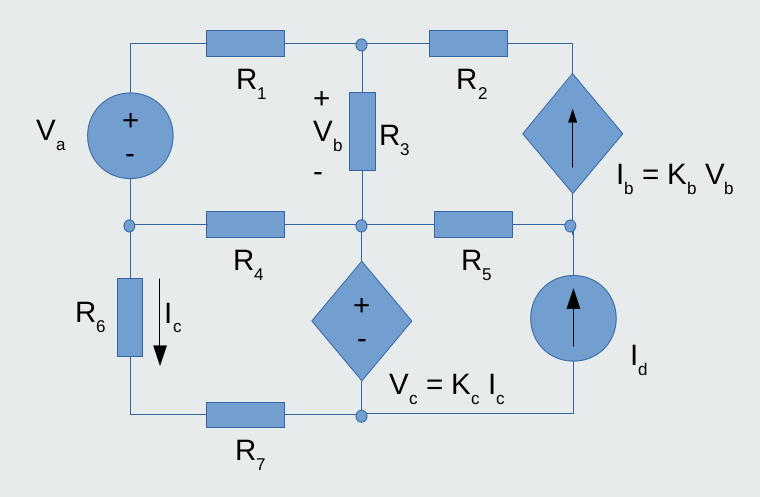
\includegraphics[width=0.8\linewidth]{Circuito.png}
    \centering
    \caption{Studied Circuit}
    \label{circuit}
\end{figure}

In Section~\ref{sec:analysis}, a theoretical analysis of the circuit is
presented. In Section~\ref{sec:simulation}, the circuit is analysed by
simulation, and the results are compared to the theoretical results obtained in
Section~\ref{sec:analysis}. The conclusions of this study are outlined in
Section~\ref{sec:conclusion}.
